\subparagraph*{Problem explaination}
The goal is the same of the previous problem, but instead of a sliding-window approach, is required to adopt a change-detection test approach.
\subparagraph*{Strategy}
In order to solve this problem we have used a change detection (CUSUM) algorithm and a bandit algorithm (UCB). At each time $t$, the UCB outputs a decision $I_t \in K$, where $K$ is a set of arms, based on its past observations of the bandit environment. The environment generates the corresponding reward of arm $I_t$, which is observed by both the bandit algorithm and the change detection algorithm. The change detection algorithm monitors the distribution of each arm, and sends out a positive signal to restart the bandit algorithm once a breakpoint is detected.

\subparagraph*{Change Detection (CUSUM)}

\textbf{Explaination:}\\

The first $M$ valid samples are used to produce the reference point.\\

Empirical mean of arm $a$ over the first $M$ valid samples $\bar{X_{a}^0}$\\

From the $M + 1-th$ valid sample on, we check whether there is a change\\

Positive deviation from the reference point at $t$ \hspace{0.2cm} $s_{a}^{+}(t) = (x_{a}(t) - \bar{X_{a}^0}(t)) - \epsilon$ \\

Negative deviation from the reference point at $t$ \hspace{0.2cm} $s_{a}^{-}(t) = -  (x_{a}(t) - \bar{X_{a}^0}(t)) - \epsilon$ \\

Cumulative positive deviation from the reference point at $t$ \hspace{0.2cm} $g_{a}^{+}(t) = \max \left\{0, g_{a}^{+}(t-1) + s_{a}^{+}(t) \right\}$ \\

Cumulative negative deviation from the reference point at $t$ \hspace{0.2cm} $g_{a}^{-}(t) = \max \left\{0, g_{a}^{-}(t-1) + s_{a}^{-}(t) \right\}$ \\

We have a change if \hspace{0.2cm} $g_{a}^{-}(t) > h$ or $g_{a}^{+}(t) > h$\\
\subparagraph*{CD-UCB}

\textbf{Pseudocode:}\\

1. Initialize $\tau_{a} = 0$ for $a\in A$ 

2. For each time $t$:\\

\hspace{0.8cm} $a_{t} \leftarrow \argmax_{a \in A}{\left\{\bar{x}_{a,\tau_{a},t} + \sqrt{\frac{2 log(n(t))}{{n_{a}(\tau_{a},t-1)}} }\right\}}$ with probability $1-\alpha$\\

\hspace{0.8cm} $a_{t} \leftarrow$ random arm with probability $1-\alpha$ \\

$n(t)$	is total number of valid samples\\

$\bar{x}_{a,\tau_{a},t}$ is the empirical mean of arm $a$ over the last valid samples\\

$n_{a}(\tau_{a},t-1)$ is the number of valid samples for arm $a$\\

3. Collect reward $r_t$\\

4. If $CD_a (r_{\tau},...,r_t) = 1$ then $\tau_a = t$ and restart $CD_a$

\subparagraph*{Results}
\begin{center}
	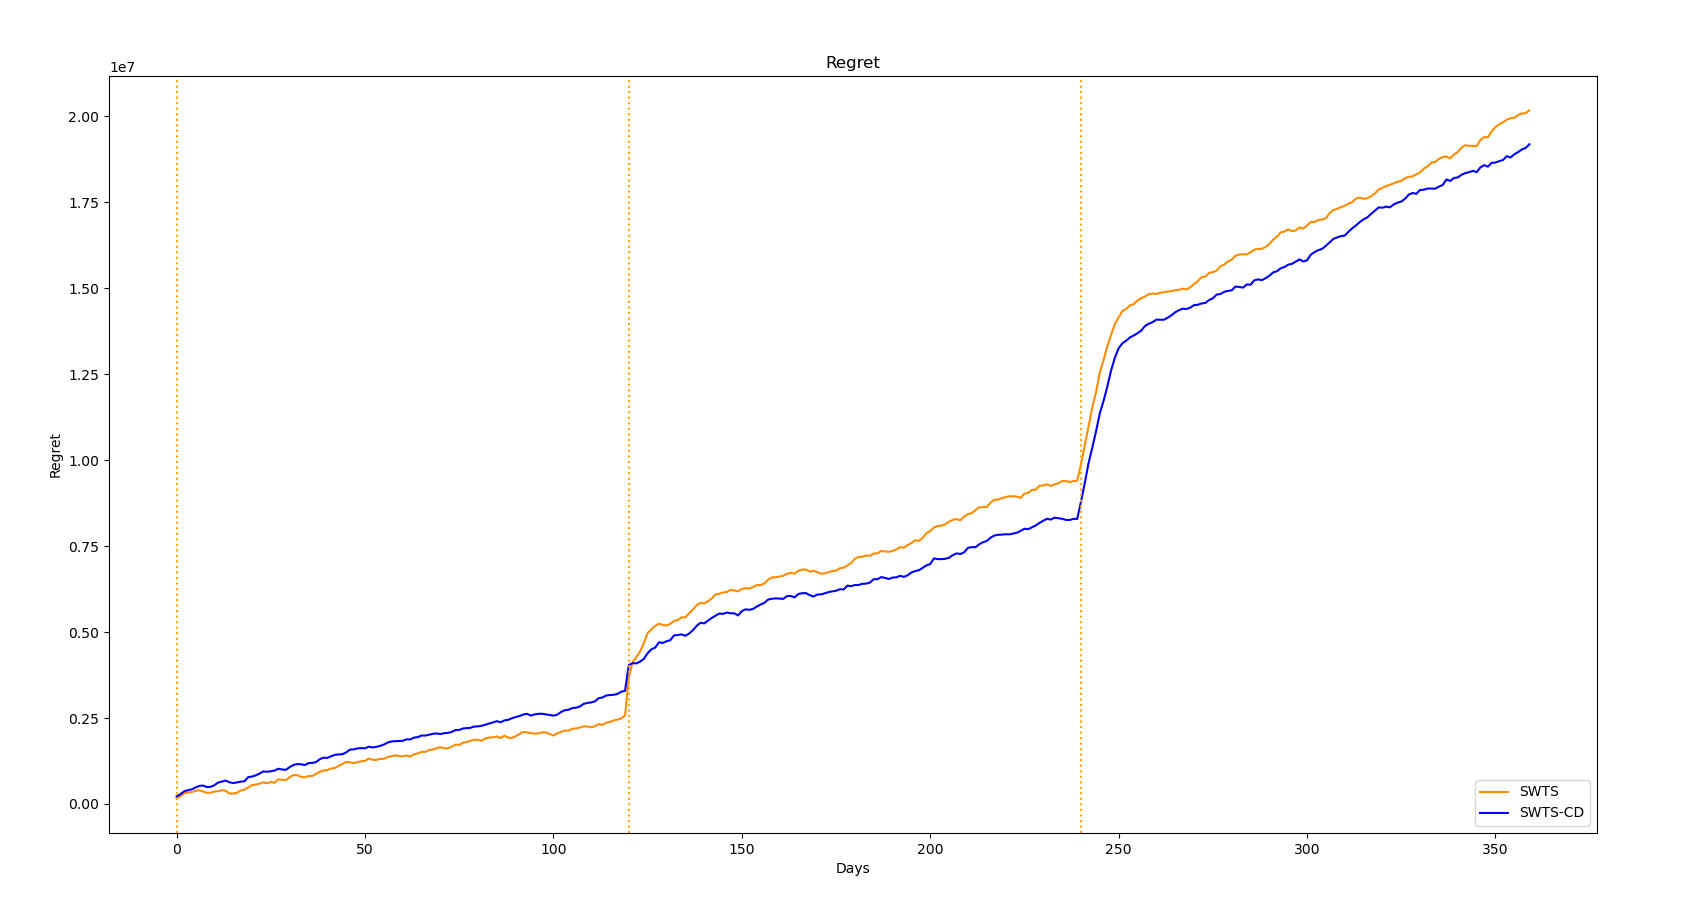
\includegraphics[scale=0.35]{Images/n8}
\end{center}
\subparagraph*{Considerations}